\documentclass[20pt, a0paper, portrait, margin=0mm, innermargin=20mm, blockverticalspace=8mm, colspace=14mm, subcolspace=6mm]{tikzposter}
\usepackage[T1]{fontenc}
\usepackage{lmodern}
\usepackage{booktabs}
\usepackage{array}
\usepackage{graphicx}
\usepackage{qrcode}
\usepackage{amsmath}
\usetikzlibrary{positioning,arrows.meta}

\definecolor{accent}{HTML}{1F5A85}
\definecolor{soft}{HTML}{EEF3F8}
\definecolor{ink}{HTML}{1F1F1E}
\definecolor{muted}{HTML}{5F5E58}
\definecolor{gbst}{HTML}{2A78D6}
\definecolor{tpp}{HTML}{EB6834}

\definecolorstyle{Project}{
  \colorlet{colorOne}{accent}\colorlet{colorTwo}{soft}\colorlet{colorThree}{white}
}{
  \colorlet{backgroundcolor}{white}\colorlet{framecolor}{white}
  \colorlet{titlefgcolor}{white}\colorlet{titlebgcolor}{accent}
  \colorlet{blocktitlebgcolor}{accent}\colorlet{blocktitlefgcolor}{accent}
  \colorlet{blockbodybgcolor}{soft}\colorlet{blockbodyfgcolor}{ink}
  \colorlet{innerblocktitlebgcolor}{white}\colorlet{innerblocktitlefgcolor}{ink}
  \colorlet{innerblockbodybgcolor}{white}\colorlet{innerblockbodyfgcolor}{ink}
  \colorlet{notefgcolor}{ink}\colorlet{notebgcolor}{white}\colorlet{noteframecolor}{accent}
}
\usetheme{Simple}
\usecolorstyle{Project}
\settitle{
  \centering\vbox{
    {\color{titlefgcolor}\bfseries\fontsize{70}{80}\selectfont Does a learned tokenizer help a small DNA model?\par}
    \vspace{0.6em}
    {\color{titlefgcolor}\Large GBST + bidirectional BERT (ChaRNABERT-style), pretrained on the human genome and compared with Transformer++\par}
    \vspace{0.8em}
    {\color{titlefgcolor}\large Omar R.A Mohamed \quad$\cdot$\quad October 2026 \quad$\cdot$\quad code, models and results: github.com/OMAR622-ai/dna-xlstm-charna (branch charna-gbst)\par}
  }
}
\newcommand{\code}[1]{\texttt{#1}}
\renewcommand{\arraystretch}{1.25}

\tikzposterlatexaffectionproofoff
\begin{document}
\maketitle[width=0.97\paperwidth, roundedcorners=0, innersep=1.4cm, titletotopverticalspace=0mm, titletoblockverticalspace=10mm]

% =============================== ROW 1 ===============================
\begin{columns}
\column{0.32}
\block{1 \quad The question}{
Most DNA language models fix in advance how a sequence is cut into ``words'': single bases,
codons or k-mers. \textbf{ChaRNABERT} (Morales-Pastor et al., 2024) instead lets the model
\emph{learn} how to cut, separately at every position (\textbf{GBST}), and reported better
results on RNA.

\vspace{0.6em}
\textbf{We ask:} does this learned reading also help a \emph{small} model of
\emph{human DNA}?

\vspace{0.6em}
\textbf{Approach:} build GBST-BERT in the DNA-xLSTM code base, train it with the DNA-xLSTM
protocol (Schmidinger et al., 2024), and compare it with the same-size \textbf{Transformer++}
that reads one base at a time.
}

\block{2 \quad The model: GBST-BERT}{
\begin{center}
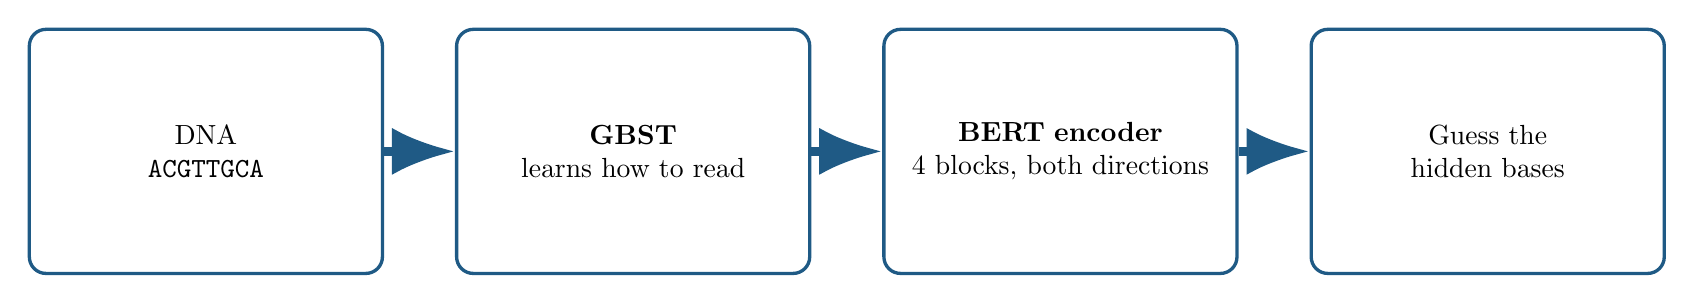
\begin{tikzpicture}[
  box/.style={draw=accent, very thick, rounded corners=6pt, fill=white, minimum height=3.1cm,
              align=center, text width=4.25cm, font=\normalsize},
  arr/.style={-{Latex[length=8mm]}, line width=3pt, accent}]
\node[box] (a) {DNA\\\code{ACGTTGCA}};
\node[box, right=0.9cm of a] (b) {\textbf{GBST}\\learns how to read};
\node[box, right=0.9cm of b] (c) {\textbf{BERT encoder}\\4 blocks, both directions};
\node[box, right=0.9cm of c] (d) {Guess the\\hidden bases};
\draw[arr] (a) -- (b); \draw[arr] (b) -- (c); \draw[arr] (c) -- (d);
\end{tikzpicture}
\end{center}

\textbf{GBST} at every position lists all blocks of 1--4 bases that contain it (10
candidates, like reading frames), scores them, and mixes them with learned weights.
Example for the first \code{T} of \code{ACGTTGCA}:

\begin{center}\normalsize
\begin{tabular}{cl}
\toprule
Size & Candidate blocks \\
\midrule
1 & \code{T} \\
2 & \code{TT}, \code{GT} \\
3 & \code{TTG}, \code{GTT}, \code{CGT} \\
4 & \code{TTGC}, \code{GTTG}, \code{CGTT}, \code{ACGT} \\
\bottomrule
\end{tabular}
\end{center}

\textbf{Encoder:} attention with RoPE and QKNorm, SwiGLU, LayerNorm (ChaRNABERT \S3.3).
\textbf{Size:} 2.1\,M parameters (256 per base, 8 heads), as the 2\,M DNA-xLSTM models.
}

\column{0.36}
\block{3 \quad Data and training}{
\textbf{Human genome hg38} (3.03 billion bases), split as in DNA-xLSTM:

\begin{center}\normalsize
\begin{tabular}{lrr}
\toprule
Split & Unique bases & Share \\
\midrule
Training & 2.33 B & 77\% \\
Validation & 0.29 B & 10\% \\
Test (never trained on) & 0.27 B & 9\% \\
\bottomrule
\end{tabular}
\end{center}

\textbf{The game (masked language modelling):} 15\% of the bases are hidden; the model must
guess them from both sides. Half of the time the reverse-complement strand is shown.

\vspace{0.4em}
\begin{center}\normalsize
\begin{tabular}{rl}
Real:   & \code{A C G T T G C A A G T C} \\
Input:  & \code{A C ? T T G C A A ? T C} \\
Answer: & \code{. . G . . . . . . G . .}
\end{tabular}
\end{center}

\begin{center}\normalsize
\begin{tabular}{ll}
\toprule
Setting & Value [source] \\
\midrule
Steps & 10,000 = 10.5 B bases [Bio-xLSTM A4] \\
Batch & 1,024 seq.\ $\times$ 1,024 bases per step \\
Optimizer & AdamW (0.9, 0.95), wd 0.1, cosine \\
LR GBST-BERT & 2e-3 (best of 4, our check) \\
LR Transformer++ & 1e-2 [Bio-xLSTM Table A3] \\
Hardware & 4 GPUs (JKU student01 / 07), fp32 \\
\bottomrule
\end{tabular}
\end{center}
}

\column{0.32}
\block{4 \quad How we test}{
\textbf{Loss:} how wrong the guesses are: average of $-\ln(\text{probability of the true base})$.
Lower is better; random guessing = \textbf{1.386}.

\vspace{0.5em}
\textbf{Accuracy:} share of hidden bases whose best guess is right, on \textbf{2,048 unseen test
sequences} (311,767 hidden bases). Both models get \emph{exactly the same} hidden positions.

\vspace{0.5em}
\textbf{References without a model:} random guessing 25\%; always guessing the most common base
(A or T) 29.4\%.
}

\block{5 \quad Engineering notes}{
\begin{itemize}
\item 24 automatic tests; checkpoints every 500 steps; every run documented on GitHub.
\item \textbf{Bug found and fixed} in the repository's genome reader: parallel reader processes
  shared one open file and sometimes read the wrong bases (0.35\% with 2 readers, up to 33\%
  with 12). Fixed with a test (841/1,024 wrong before, 0 after); runs resumed from a clean
  checkpoint. Test DNA never leaked into training.
\item Training moved between servers mid-run and resumed exactly from a checkpoint.
\end{itemize}
}
\end{columns}

% =============================== ROW 2: results ===============================
\block{6 \quad Results: validation loss for every trained learning rate, and the final test}{
\begin{center}
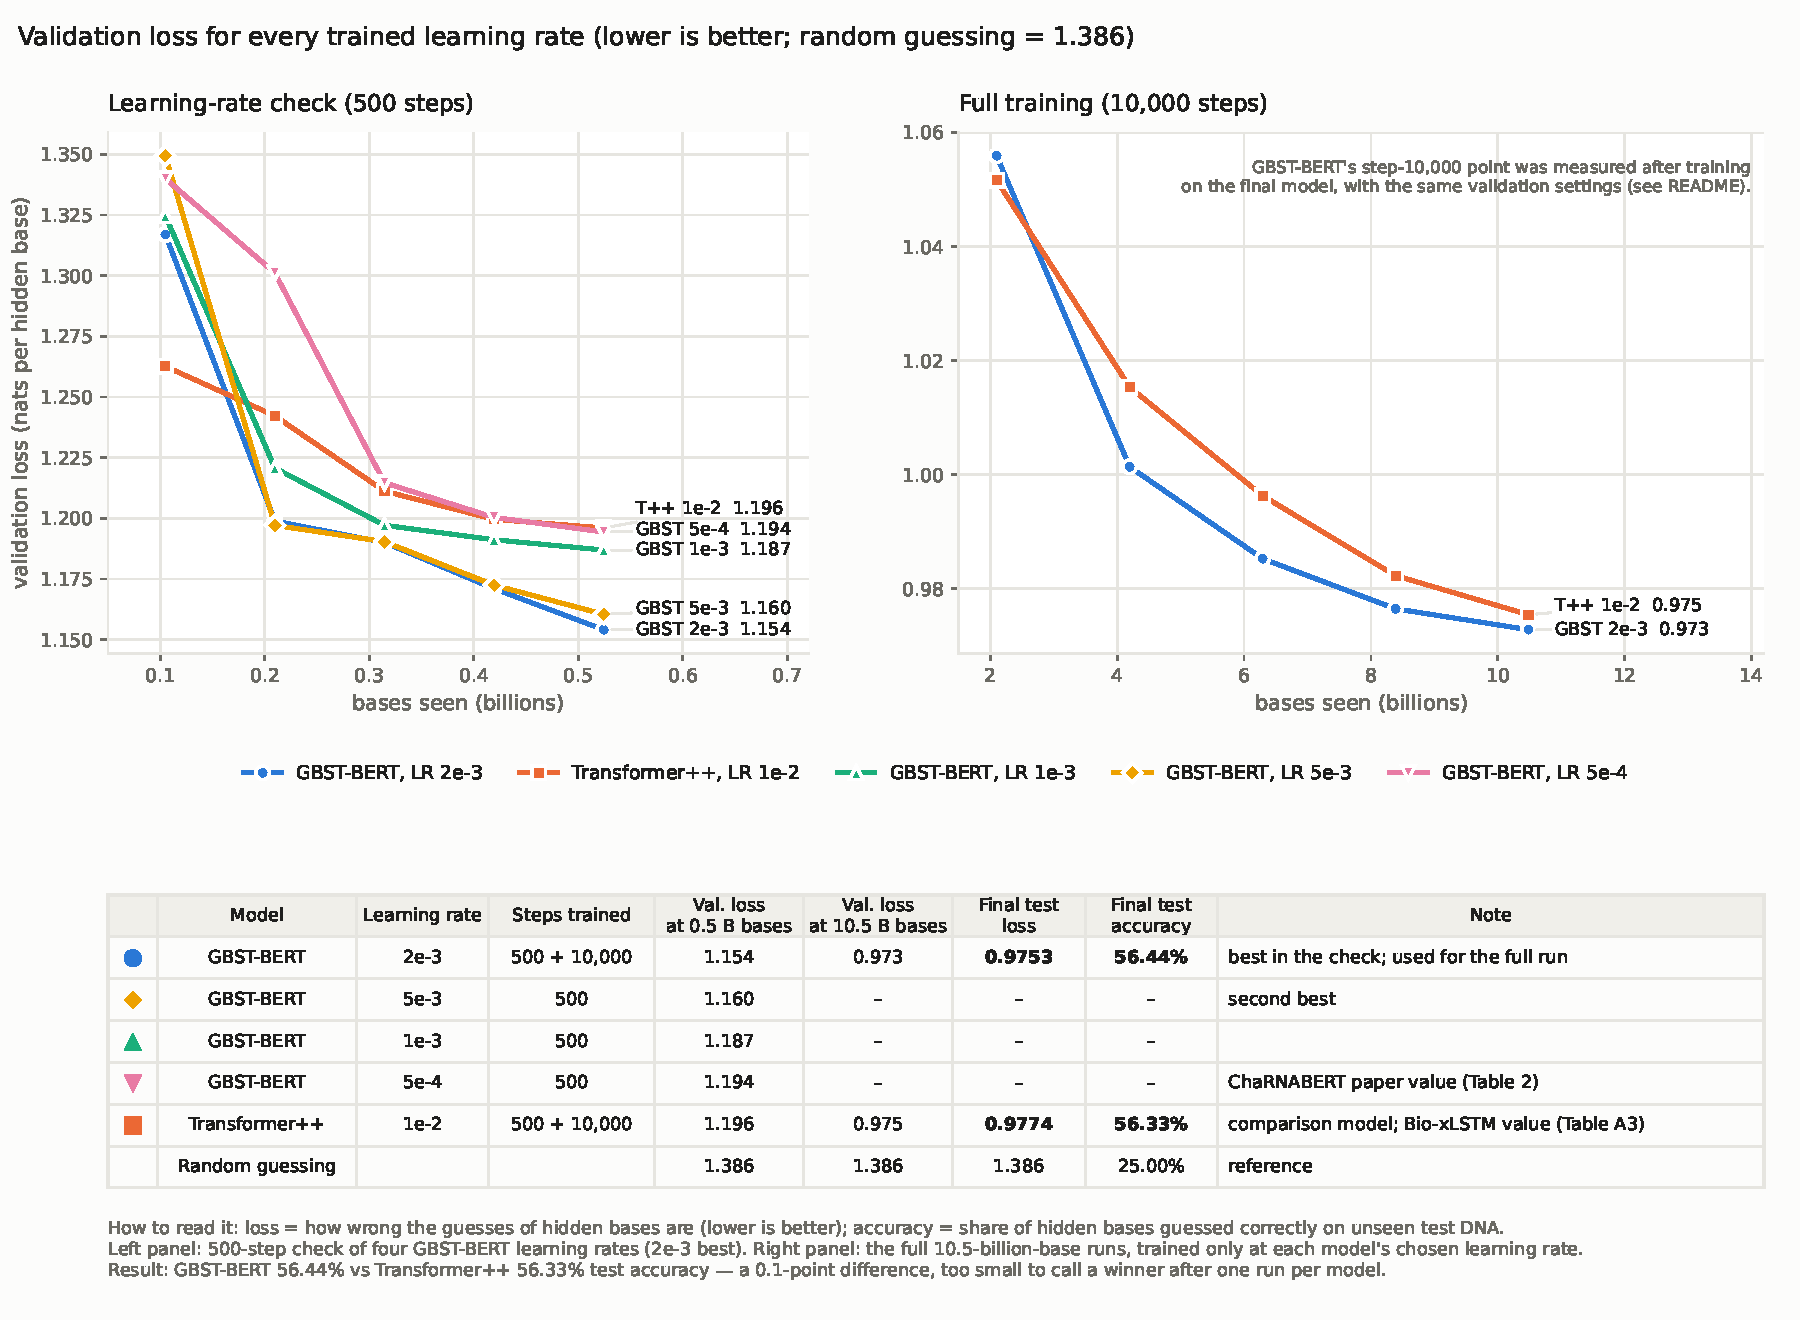
\includegraphics[width=0.70\linewidth]{figures/curves_table.pdf}
\end{center}
}

% =============================== ROW 3 ===============================
\begin{columns}
\column{0.34}
\block{7 \quad What GBST learned}{
Share of GBST's weight on blocks of 1 / 2 / 3 / 4 bases (8 sequences, different chromosomes):

\begin{center}\normalsize
\begin{tabular}{lc}
\toprule
Model & 1 / 2 / 3 / 4 bases \\
\midrule
500 steps, LR 5e-4 & 72 / 22 / 5 / 1\% \\
500 steps, LR 2e-3 & 98 / 2 / 0 / 0\% \\
Full run, step 2,000 & 99.8 / 0.1 / 0 / 0\% \\
\textbf{Final model} & \textbf{98 / 2 / 0 / 0\%} \\
\bottomrule
\end{tabular}
\end{center}

On human DNA, GBST learned to read \textbf{almost only single bases}; each base still sees its
neighbours through the convolution before the blocks. GBST-BERT therefore behaves close to a
one-base-at-a-time model.
}

\column{0.36}
\block{8 \quad Conclusions}{
\begin{itemize}
\item Both 2\,M models learned human DNA well: \textbf{56\% accuracy} (random 25\%), test loss
  $\approx$\textbf{0.975}, in the range of the published 2\,M models ($\approx$0.96--1.03).
\item GBST-BERT was ahead for most of the training, but finished only \textbf{0.1 points}
  ahead (56.44\% vs 56.33\%) --- too small to say GBST helps.
\item GBST learned to use mostly single bases, which explains why the models end so close.
\item On RNA, ChaRNABERT also found only small gains (e.g.\ loss 0.498 vs 0.508, Table 2).
\end{itemize}

\textbf{Caveats:} one run per model; only GBST-BERT's learning rate was tuned; the models also
differ in normalization.
}

\column{0.30}
\block{9 \quad Next steps}{
\begin{enumerate}
\item \textbf{Clean test of GBST:} the same model with GBST replaced by a plain lookup table
  (\code{TOKENIZER=embedding}), same settings.
\item \textbf{Biology tasks:} Nucleotide Transformer benchmark (18 tasks: promoters, enhancers,
  splice sites, histone marks) --- code ready and tested.
\item Repeat runs with other seeds; MLM vs UL2.
\end{enumerate}

\vspace{0.2em}
\begin{center}
\qrcode[height=4.2cm]{https://github.com/OMAR622-ai/dna-xlstm-charna/tree/charna-gbst}\\[0.3em]
{\normalsize Code, models, results (private repository)}
\end{center}
}
\end{columns}

\end{document}
